\chapter[G Ramachandran -- My reminiscences]{G Ramachandran\break -- My reminiscences}\label{chap25}

\Authorline{V. Ravishankar}

\authinfo{Department of Physics\\ IIT Delhi}


Professor G. Ramachandran, GR as we called him, was my teacher who had the greatest influence on my life as a physicist. I had the opportunity to get to know him when I was an undergraduate student, still a “babe in woods”. That was in 1976, when he visited our college to deliver a lecture on quantum mechanics. These days, we teach quantum mechanics to students very early, but back then, one had to wait until one got a chance to enroll in M.Sc.\ To us, the undergraduates, relativity was tough, but quantum mechanics was formidable.

While we looked forward to a popular lecture, he went on directly to tell us about measurements, standard deviations (what we call uncertainty), and the limitations imposed by quantum mechanics on standard deviations of measurements involving position and momentum (the uncertainty principle). If I remember correctly, since this necessitates the concept of state, he introduced it without much ado. The treatment was prescriptive, and not descriptive.  Thus, here was a baptism which was shorn of all ``philosophical" frills, and also of all those confusing notions such as Heisenberg's thought experiment. That was wise on his part. Students appreciate those concepts much better after a good exposure to the subject. Hopefully.

But at that moment, it was a jolt.  But it was also a great relief. For, one can then actually start working. That is, calculate. In about three hours --- the duration of his discourse, he had introduced the Schr\"{o}dinger equation, and even worked out the oscillator problem to some extent. They were interspersed with generous doses of insights and words of caution. The attendance in the first lecture was close to 50. In the next one, on the very next day, it was about ten.

Thus started my interaction with GR in whom I found a source of a no nonsense and direct approach to physics. Also, here was a person with a great capacity to put up with my very many nonsensical questions. Meeting him became an almost regular affair. Though I could follow little, I would still listen to the discussions he had with his students: M. V. N. Murthy, Keshava Murthy and K. Venkatesh. On their part, they did put up with me; in fact, even indulged me. They treated me as a member of their group. Such spontaneous generosity is rare. University of Mysore proved to be much more attractive than IIT Bombay when it was time for me to do my post graduate studies.

The story could go on. But we do get a glimpse of the teacher in GR who would welcome any one who approached him for learning physics. Great was his passion and energy. In his regular courses in the university, classes typically started about 20 minutes late, and ended typically about 180 minutes later than when it was expected to be. We ran a marathon with him, week after week. Once, we were thrown out of the class room because he had lectured for more than four hours and the office staff could wait no longer. The lectures were spontaneous, calculations were done extempore on the board, and the material covered was enough to keep us busy for yet another three hours after the class.

His love for physics was abiding, but we seldom saw any hero worship.  I believe that this got rubbed on to us too. Especially when it came to research.

Now for the kind of research problems that GR was wont to tackle. Here, one may state that two themes characterised most of his work. One was a practical implementation of the slogan -- “Spin is in. Spin is fun”. He was deeply interested in nuclear interactions involving the spin degree of freedom. You have to just go through his papers in Nuclear Physics (the journal) on nuclear reactions, and subsequent works on parity violations, and a much later work on EPR violation too. Some of them had collaborators (including students) and others, none. He even attempted to understand the hydrogen bond in terms of Racah coefficients when he was in the group of G. N. Ramachandran in the molecular biophysics department at Indian Institute of Science. He showed me his notes once, and though it did appear like a really long shot, its very “audacity” was highly refreshing.

So, GR was The "spin doctor". This brings us to the second theme that permeated his research. That was diagnostics. I could be wrong here. But I always felt that GR had no great interest -- perhaps even the gumption -- to work on new “theories” or models\footnote{There is at least one delightful exception. Together with the legendary G. N. Ramachandran and a colleague, Tagare, he proposed a model involving tachyons to explain the stability of electron. The electron is looked upon, classically, as a sphere spinning about its axis. In fact, they recovered its classical radius.  He was no believer in tachyons, though.}. Instead, he preferred to exploit his enormous mastery over the theory of angular momentum to use it in a variety of situations --- mostly nuclear interactions with pions and photons — to get signatures that would validate a theory or a model. Spin effects typically manifest as interference terms in amplitudes. The insight was in noting that small effects are better discerned through these interference terms, since then the small term gets multiplied by a much bigger term.  The emphasis was, therefore, not on the details of a process. He was, for example, content to use the so called plane wave impulse approximation, though it was clear by the time I joined him for Ph.D. that it needed refinement in terms of distortion of the plane wave, and also required the inclusion of final state interactions. GR was disinterested in these new developments to the point of appearing lethargic. This did not, however, substantially impact the validity of his results. But it did make it rather difficult to compare our numbers with experiments. In other words, our calculations yielded numbers which were indicative. They were not definitive.

But the positives of his approach overwhelmingly override the drawbacks. When you focus on a symmetry, or its violation, it is necessary not to miss the wood for the trees. As we learnt, it happens many a time that a brute force calculation mixes up the inessential details of phenomenology with the essential physics present in the problem. His method was to separate the universal geometric aspects from the differences that accrue due to the employment of different models. Evidence for such an overarching approach may be seen even in one of his earlier papers on rearrangement collisions, which he wrote together with Alladi Ramakrishnan and V.\ Devanathan.

GR's works on processes with spin degrees of freedom flowered into a strong interest in the formalism of density matrix itself.  So there were papers, written together with Murthy, where they advocated employing the standard generators of $SU(N)$ for representing of a spin density matrix\footnote{Somewhat surprisingly to me, they employ the matrices in the form given by Itzyksohn and Neuenberg, and not the ones given by Gell-Mann, but that is of little importance.}.  This work merits a couple of more sentences. The novelty was in the fact that since the matrices are fixed, they represent different sets of operators, unitarily related to each other, every time we write $\rho$ in a new basis.  With this unorthodox approach, several results could be obtained in a very elegant form. Subsequently, there was a return to the basis provided by the irreducible tensors of the group $SU(2)$. We studied the geometry of these irreducible tensors in some detail which, in turn, illuminated several aspects of the geometry of spin density matrices themselves. This formal study had a practical application: identifying observables that determine the reaction amplitudes fully in the spin space\footnote{There is an interesting historical context here. We came to know, much later, that $SU(N)$ matrices had already employed been used by Von Neumann in 1936, purely as a formal means. As to the geometry of irreducible tensors, it seems to have been rediscovered several times, in different languages -- before and after our work. I got an occasion to trace this backwards first to the work of Biedenharn who refers to Bacry, and whose work was itself preceded by the first discovery, made by Majorana. I also learnt that Schwinger's monumental work on angular momentum was inspired by Majorana's result. I have, subsequently, seen at least two papers in which the representation is arrived at.}. This theme was continued in his collaboration with Sandhya where they looked, both together and independently, at complete determination of reaction amplitudes in some very concrete examples involving nuclear processes. These works did not need the earlier results and they had devised more efficient and direct methods.  I notice that there were a few more papers on the same theme.

I have not checked, but I would believe that GR continued this approach to research long after I had moved out of Mysuru, even after he had joined the Indian institute of astrophysics, where he started working on solar spectrum. It must be mentioned that faculty at IIAP have spoken of his inspiring presence in their institute.

Isolation of talent can have undesirable effects, even on a person who is otherwise strong. While his presence in the University of Mysore was a boon to so many of us, he did have to pay a price. He got rather cut off from other developments in particle physics. This arose, in part, because he had paid scant attention to renormalisation in field theories\footnote{he called them pathological --- a hangover of the feeling of early sixties.}. This, perhaps, impeded his fuller appreciation of the standard model, apart from meager interaction with other particle physics phenomenologists. This is, of course, not a blemish. For,``the ocean of learning is so deep that even the Goddess of learning hangs on to her Veena for support". He towered over many of his peers, which went without acknowledgement, many a time. We were aware of that, and he himself felt it keenly, at times.

GR was, in a sense, an iconoclast in physics. As I said earlier, we saw little trace of hero worship of great physicists in him. In his personal life, which he kept so easily and clearly compartmentalised from his profession, he was devout and religious. He diligently performed his daily rituals, and had great reverence for the scriptures. It contrasted nicely with his often made remark, ``all that is printed is not true" when it came to physics. He saw no contradiction in this. It was, perhaps, merely his way of balancing his keen critical faculty with his equally deep spiritual needs and cultural heritage (some would call it a baggage).  He almost shunned discussions on philosophy of science, but relished discussions on Indian philosophy. We spent many an hour on this. Even here, he was interested in appreciating it as a means of spiritual wisdom. He found the logical aspects mildly interesting.

Great as his influence on us was, the umbilical cord that tied us --- his students --- to him, had to be necessarily cut. On a personal note, this was not painless, even though he himself had prepared me well enough to be independent. In any case, his students went on to do many things. Particle physics, dynamical systems, reactor physics, quantum optics, quantum information and condensed matter physics are some of the names that immediately pop up - a testimony to his mentor-ship. He endeavored to teach us to think. He was a giant tree, but his students did not need to be under his shadow.

Finally, I should end up by mentioning that my suppers during my PhD days were almost evenly distributed between my own home and GR's home. I got to know his family. His wonderful, wonderfully patient wife Ms Seetha Lakshmi, his mother -- who did wield her authority over him, with good reason, his children and, of course, his brother Vishwanathan who also showered his affection on me.

It is no wonder that we cherish his memory. Even those who came in touch with him for brief periods. He touched every ones heart.
\medskip

\begin{wrapfigure}{l}{0mm}%
\vspace{-4\baselineskip}
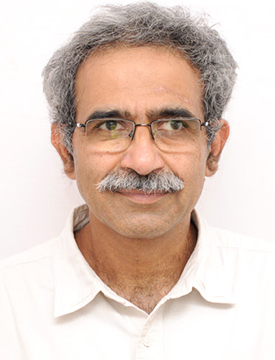
\includegraphics[scale=.3]{authorsphotos/V_Ravishankar.jpg}
\end{wrapfigure}%
\noindent
\textbf{Dr.\ V. Ravishankar} obtained the M.Sc.\ degree in 1981 and Ph.D. in 1987 from Mysore University. He worked for Ph.D. under the guidance of Prof.\ G.\ Ramachandran. After a year as Postdoctoral Fellow at TIFR, Mumbai, he joined the Physics Department, IIT Kanpur, in 1989. In 2014, he moved to the Physics Department, IIT Delhi, as a Professor in the Department.


%~ \newpage

%~ \centerline{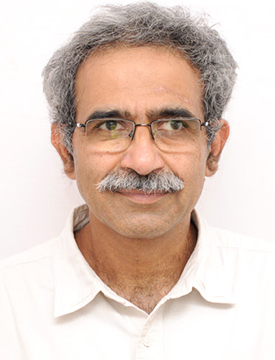
\includegraphics[scale=.3]{authorsphotos/V_Ravishankar.jpg}}
%~ \smallskip

%~ \authbio{V. Ravishankar}
%~ \bigskip

%~ \noindent
%~ \textbf{Dr.\ V. Ravishankar} obtained the M.Sc.\ degree in 1981 and Ph.D. in 1987 from Mysore University. He worked for Ph.D. under the guidance of Prof.\ G.\ Ramachandran. After a year as Postdoctoral Fellow at TIFR, Mumbai, he joined the Physics Department, IIT Kanpur, in 1989. In 2014, he moved to the Physics Department, IIT Delhi, as a Professor in the Department.
